% This must be in the first 5 lines to tell arXiv to use pdfLaTeX, which is strongly recommended.
\pdfoutput=1
% In particular, the hyperref package requires pdfLaTeX in order to break URLs across lines.

\documentclass[11pt]{article}

% Remove the "review" option to generate the final version.
\usepackage[]{acl}

% Standard package includes
\usepackage{times}
\usepackage{latexsym}
%booktabs
\usepackage{enumitem}
\usepackage{booktabs}
\usepackage{graphicx}
\graphicspath{ {./figures/} }
\usepackage{hyperref}
\usepackage{amsmath}

% For proper rendering and hyphenation of words containing Latin characters (including in bib files)
\usepackage[T1]{fontenc}
% For Vietnamese characters
% \usepackage[T5]{fontenc}
% See https://www.latex-project.org/help/documentation/encguide.pdf for other character sets

% This assumes your files are encoded as UTF8
\usepackage[utf8]{inputenc}

% This is not strictly necessary, and may be commented out,
% but it will improve the layout of the manuscript,
% and will typically save some space.
\usepackage{microtype}

% If the title and author information does not fit in the area allocated, uncomment the following
%
%\setlength\titlebox{<dim>}
%
% and set <dim> to something 5cm or larger.

\title{Trustworthy Bias Measures for Language Models and Word Embeddings\\Natural Language Processing 2}

% Author information can be set in various styles:
% For several authors from the same institution:
% \author{Author 1 \and ... \and Author n \\
%         Address line \\ ... \\ Address line}
% if the names do not fit well on one line use
%         Author 1 \\ {\bf Author 2} \\ ... \\ {\bf Author n} \\
% For authors from different institutions:
% \author{Author 1 \\ Address line \\  ... \\ Address line
%         \And  ... \And
%         Author n \\ Address line \\ ... \\ Address line}
% To start a seperate ``row'' of authors use \AND, as in
% \author{Author 1 \\ Address line \\  ... \\ Address line
%         \AND
%         Author 2 \\ Address line \\ ... \\ Address line \And
%         Author 3 \\ Address line \\ ... \\ Address line}

\author{Juno Prent \\
  Universiteit van Amsterdam \\
  \texttt{11915307@uva.nl} \\\And
  Wu Wang Yang \\
  Universiteit van Amsterdam\\
  \texttt{ID:14269244} \\\And
  Wenkai Pan \\
  Universiteit van Amsterdam \\
  \texttt{wenkai.pan@student.uva.nl}}

\begin{document}
\maketitle

\begin{abstract}
This study examines the reliability and validity of the Word Embedding Association Test (WEAT) as a measure of gender bias, applying a selection of experiments on it that have not been previously reported on. We employ pretrained word2vec embeddings in our experiments, as WEAT is specifically designed for static embeddings. The findings indicate that WEAT's measurements consistently detect a similar gender bias present in these embeddings. Moreover, the results demonstrate consistency with several other bias measures, showing WEAT to be reliable and valid.
\end{abstract}

\section{Introduction}
In everyday language, many biases of different types occur, such as gender, race or religion. This can lead to a perpetuation of incorrect stereotypes or other misinformation, among other negative effects. Unfortunately, these language biases are also captured by natural language processing (NLP) models and data. 

Here, the focus will lie on the detection of gender bias in static word embeddings from word2vec\cite{word2vec}. To do so, the WEAT\cite{weat} bias metric is used, as implemented from the WEFE\footnote{\url{https://pypi.org/project/wefe/}} Python package. These bias scores will be analyzed on two different aspects. These are reliability, so whether the measurements are consistently similar, and validity, which determines whether a certain bias score for embeddings means that these are actually biased, or whether this score might actually be influenced by other factors.

The analysis of WEAT's bias measurements leads to the following research questions:
\begin{enumerate}
    \itemsep-0.5em
    \item What is the reliability of WEAT's bias measurements?
    \item What is the validity of WEAT's bias measurements?
\end{enumerate}

These were answered through experiments pertaining to WEAT's reliability and validity, assessing how consistent its measurements are and how they compare to those of different bias metrics. From these experiments, it was found that WEAT is indeed a reliable and valid bias metric.

\section{Background}
In recent years, the issue of bias in language models and word embeddings has received significant attention. Several studies have highlighted the presence of gender biases in these models and their potential negative implications for perpetuating stereotypes and misinformation. Gonen and Goldberg \cite{gonen-goldberg-2019-lipstick} conducted a comprehensive analysis of debiasing methods. They demonstrated that existing debiasing techniques may mitigate explicit gender bias in word embeddings, but fail to address the underlying systematic biases. This highlights the need for effective and reliable bias measurement methods.

Evaluation of gender bias in word embeddings is a crucial aspect of addressing bias in language models. However, Orgad and Belinkov \cite{orgad-belinkov-2022-choose} identified flaws in gender bias evaluation methods. They discussed the limitations of the popular WEAT and proposed alternative evaluation approaches to provide a more nuanced understanding of gender bias in word embeddings. This highlights the importance of critically examining bias measurement methods and exploring alternative metrics.

Ethayarajh, Duvenaud, and Hirst \cite{ethayarajh-etal-2019-understanding} delved into the issue of undesirable word embedding associations. They highlighted the presence of unintended associations between protected attributes (e.g., gender, race) and other words in word embeddings. Their work emphasized the need to develop measures that not only capture explicit biases but also account for implicit associations and undesirable connotations present in word embeddings.

Guarding against biases in protected attributes is another significant concern. Ravfogel et al. \cite{ravfogel-etal-2020-null} proposed the Iterative Nullspace Projection method. Their approach focused on protecting sensitive attributes, such as gender or race, by iteratively projecting the embeddings onto a null space to remove associations with the protected attribute. This work highlights a potential technique to mitigate biases associated with protected attributes in word embeddings.

Drawing from the insights of these studies, this research aims to address the limitations of existing bias measurement methods and explore the reliability and validity of WEAT as a measure of gender bias. Additionally, we aim to investigate the consistency of WEAT's measurements and compare them with other bias metrics. By doing so, we aim to provide a deeper understanding of gender biases present in word embeddings and contribute to the development of more effective and trustworthy bias measurement techniques.

\section{Approach}
\subsection{WEAT}
WEAT is a bias metric aimed at detecting bias within static word embeddings. As its input, it takes two different types of sets: attribute sets, which can be gendered words, such as pronouns or names, and target sets, which are supposed to be gender-neutral words, such as occupational terms. 

To obtain its output, WEAT then calculates the cosine similarity between the attribute and target sets. A higher value for the cosine similarity can be interpreted as a higher level of bias, as this means there is more of an association between the embeddings of the gender-neutral and gendered terms. This, of course, is often not desirable.

\subsection{Assessment methods}
\subsubsection{Reliability}
To test the reliability, the choice was made to use the method of internal consistency. Internal consistency is a measure used to assess the consistency and reliability of a test or measurement instrument, such as WEAT. It examines the extent to which the items or components within the test are measuring the same underlying construct or concept. For these experiments, random samples of various sizes of the target and attribute concept lists were taken and their effect sizes compared to an established baseline.

Employing this internal consistency reliability measure gives insight into whether WEAT is consistently measuring the desired associations between target and attribute concepts, namely gender bias. Ideally, the effect size for randomized samples is still close to that of the baseline, given a sufficiently large sample size. If this isn't the case, WEAT might be overly dependant on specific items to obtain its results, leading to very different results when these items are not present. Higher levels of internal consistency provide evidence for the reliability of the metric.

\subsubsection{Validity}
To test the validity of WEAT, we chose to employ convergent validity. Convergent validity is a type of validity assessment that examines the degree to which a test or measurement correlates with other measures or indicators that are expected to assess a similar concept, in this case bias. In the context of testing the validity of WEAT, we employ convergent validity to evaluate whether the results of WEAT align with other measures that assess similar associations between target and attribute concepts. For this, the measures Word Analogy Testing and Word Similarity Comparison were used.

Word Analogy Testing is a method used to evaluate the performance of word embeddings or language models in capturing semantic relationships between words. It involves assessing the ability of a model to accurately complete analogical relationships in the form of word analogies and can also be used to assess gender bias in word embeddings or language models. To evaluate the gender bias, we construct analogy questions that specifically target gender-related associations. An example would be "father is to son as mother is to \_\_".

Word Similarity Comparison is the process of quantifying the similarity between two words based on their semantic or contextual similarity. It involves measuring how closely related or similar two words are in terms of gender association.

To support this experiment, a downstream task was conducted: semantic textual similarity for bias (STS-B)\cite{sts-b}, a common benchmark for assessing how NLP models measure the semantic similarity between pairs of texts. Here, a modified version was used, as used in the assignment notebook. It compares similarity scores between three pieces of text. For example, if we have two differently gendered sentences A and B, along with a neutral sentence C, similarity scores of A and C with B and C can be compared. The gender bias of the neutral term in C is then the difference in the similarity averaged over a set of template sentences. Figure \ref{fig:STS-B} further illustrates this approach.

\begin{figure}[htbp]
  \centering
  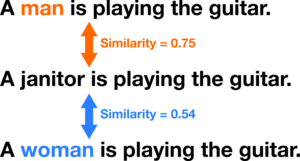
\includegraphics[width=0.4\textwidth]{figures/STS-B.png}
  \caption{Intuition behind STS-B}
  \label{fig:STS-B}
\end{figure}

\subsection{Word embeddings}
For this undertaking, the decision was made to utilize word2vec embeddings that were pretrained specifically on the Google News corpus. This particular model, known as \textit{word2vec-google-news-300}, is a pretrained word embedding model developed by Google and trained on an extensive collection of Google News articles. It encompasses word vectors with a dimensionality of 300. To access this pretrained word2vec modem, \textit{downloader} from the \textit{Gensim} library was used.

\section{Experiments and results}
\subsection{WEAT baseline}
To obtain a baseline for WEAT that could be used for further comparisons, WEAT was applied to the word2vec embeddings. Four lists of gendered words and associated concepts were created, each with 32 items. Their categories were male names, female names, family relationships, and occupations. For the names, the top 32 most common names per gender in the past century in the USA\footnote{\url{https://www.ssa.gov/oact/babynames/decades/century.html}} were chosen. For simplicity, WEAT is conducted using the aforementioned \textit{WEFE} package, which is developed for the evaluation and analysis of fairness in word embeddings. It provides a range of tools and metrics to measure and quantify different aspects of bias and fairness in word embeddings. The reason why we chose WEFE is because it comes with handy functions to assess various types of biases, such as gender bias, racial bias, and other forms of social bias, in word embeddings.

WEAT yielded an effect size of approximately 1.22. The effect size quantifies the magnitude of the association between the target and attribute concepts in WEAT. A larger effect size suggests a stronger association. In this case, the effect size implies that the difference between the means of the target word embeddings in the two attribute categories is well over one standard deviation. This suggests a notable distinction between the two sets and indicates a substantial effect or relationship, that being a relatively strong gender bias.

\subsection{Reliability}
To measure the reliability of the WEAT measurement, an internal consistency experiment was done in which randomized samples of varying sizes, ranging from 4 to 24, were taken of each of the four concept lists. This was done 10.000 times for each sample size, giving a total of 210.000 sets of four randomized samples. 

WEAT was then applied on these samples each time to determine its effect size and how close it was to the previously established baseline. The average effect size obtained for each sample size, as well as the baseline's effect size, is visualized below in Figure \ref{fig:avg effect sizes}.

\begin{figure}[htbp]
    \centering
    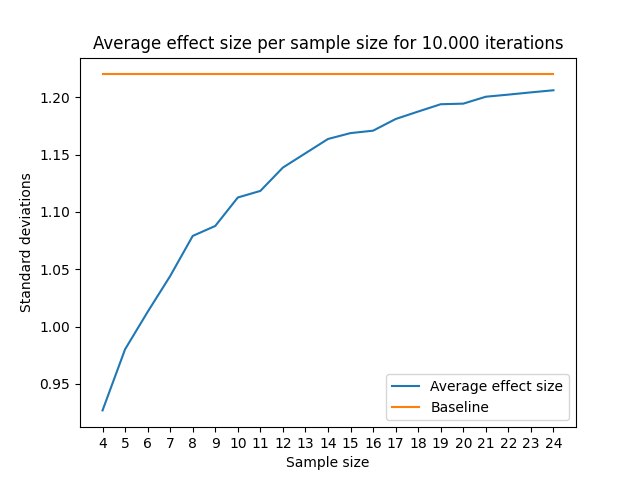
\includegraphics[scale=0.52]{figures/avg_effect_sizes.png}
    \caption{}
    \label{fig:avg effect sizes}
\end{figure}

\subsection{Validity}
\subsubsection{Word Analogy Testing}
For Word Analogy Testing, we defined a list of 10 analogies ourselves which can be found in the notebook. The results were obtained as follows: if the model predicts an analogy as expected then the result is recorded as the index of this sample. Otherwise, it is recorded as 0. For example, if the data set has 4 samples, in the case where the first three samples are correctly predicted and the last sample is predicted wrong, the results will be [1,2,3,0].

\subsubsection{Word Similarity Comparison}
For Word Similarity Comparison, a list of gendered pairs and gender-neutral pairs are defined, each containing 78 pairs. Results are also recorded in the same way as that in Word Analogy Testing. 

\subsubsection{Evaluation}
To analyze the outcomes of the aforementioned tests, we utilized the Kappa score as a means to assess the level of agreement between the two evaluations. This is a statistical measure employed to gauge the agreement between two raters or evaluators categorizing items into distinct categories. The Kappa score goes from 0 to 1, with 1 signifying complete agreement.

Here, the computation of the Kappa score is done using the \textit{cohen\_kappa\_score} library in \textit{sklearn} package. With this, a score of approximately 0.76 was obtained. This falls in the 0.61-0.80 segment, which indicates that there is a substantial level of agreement.  

\subsubsection{STS-B}
For this undertaking, we utilized a pre-existing dataset comprising a total of 276 samples\footnote{\url{https://drive.google.com/drive/folders/1PQlC1P1zhhgtGc7dSD5UcIB9IZtEzPi7}}. Each sample consists of three sentences that incorporate either the term "man," "woman," or an occupational descriptor, as described previously. The results show that 69.9\% of the input samples favour the male concept.

\section{Discussion}
\subsection{Reliability}
When looking at the results of the internal consistency experiment seen in Figure \ref{fig:avg effect sizes}, the consistency of WEAT's measurements becomes apparent immediately. Keeping in mind the baseline's effect size of around 1.22 standard deviations, it can be seen that this value is quickly approached as the sample size increases, with only the very lowest sizes being far off the baseline. When the sample size is 16, meaning exactly half of each concept list is randomly sampled each iteration, the difference with the baseline is less than 0.05 already.

From this, it can be concluded that WEAT's measurements are indeed reliable. There is no overdependence on specific input elements and measurements are consistent with the baseline over large amounts of iterations, for differing sample sizes. As a bias metric should be reliable to be of any importance, this does not come as a surprise.

\subsection{Validity}
The approximately 0.76 Kappa score from the convergent validity experiment suggests that the two additional measures substantially align with each other on the assessment that the pretrained word2vec embeddings possess gender bias. This also aligns with the outcomes of WEAT's measurement of the same embeddings.

The outcome of the downstream STS-B task further solidifies these findings. In any unbiased setting, there would not be such a stark preference for male concepts in words that are supposed to be gender-neutral in meaning. This should thus have lead to only a theoretical 50\% preference for the male concepts, which is far lower than was obtained. As this indication of gender bias is also in line with WEAT, it can be concluded that there are many signs that WEAT's bias measurements are valid. As this is desired for a bias metric such as WEAT, this does not come as a surprise either.

\subsection{Future work}
As the focus on bias detection is a recent development, it is not quite clear which bias metrics can be fully trusted yet\cite{norwegian_salmon}. As such, future work might do well to focus on establishing whether bias metrics other than WEAT, such as Embedding Coherence Test\cite{ect}, can also be considered reliable and valid. Doing so for a wider selection of bias metrics will result in a clearer overview of trustworthy methods for detecting biases for a wider array of use cases.  

\section{Conclusion}
To summarize, several experiments were performed with the bias metric WEAT to assess it on two aspects, those being the reliability and validity of its gender bias measurements. From the results, it became clear that these measurements are consistent among different randomized settings and also in line with the bias measurements of several other bias metrics. As such, it can be concluded that WEAT is indeed a reliable and valid metric for gender bias.  

\bibliographystyle{plain}
\bibliography{custom}

\section*{Appendix}
\subsection*{Contribution overview}
Juno: 
\begin{itemize}
    \item Did the tutorial notebook, except for Q1.3. Wrote the PDF file about it
    \item Wrote reliability experiment
    \item Implemented STS-B data set
    \item Wrote Introduction, all sections relating to reliability experiment, Discussion and Conclusion
    \item Wrote other small parts, restructured/rewrote large parts of our original report to adhere to rubric structure
\end{itemize}

Wangyang: 
\begin{itemize}
    \item Did the tutorial Q1.3
    \item implementation for WEAT for pretrained word2vec embeddings
    \item Designing and coding for validity experiment
    \item Wrote Abstract, WEAT and word embeddings sections in Approach, all sections relating to validity experiment
\end{itemize}

Wenkai:
\begin{itemize}
    \item Wrote Background section
\end{itemize}

\end{document}